% This must be in the first 5 lines to tell arXiv to use pdfLaTeX, which is strongly recommended.
%\pdfoutput=1
% In particular, the hyperref package requires pdfLaTeX in order to break URLs across lines.

\documentclass[11pt]{article}

% Remove the "review" option to generate the final version.
\usepackage{acl}

% Standard package includes
\usepackage{times}
\usepackage{latexsym}

% For proper rendering and hyphenation of words containing Latin characters (including in bib files)
\usepackage[T1]{fontenc}
% For Vietnamese characters
% \usepackage[T5]{fontenc}
% See https://www.latex-project.org/help/documentation/encguide.pdf for other character sets

% This assumes your files are encoded as UTF8
\usepackage[utf8]{inputenc}

% This is not strictly necessary, and may be commented out,
% but it will improve the layout of the manuscript,
% and will typically save some space.
\usepackage{microtype}

% If the title and author information does not fit in the area allocated, uncomment the following
%
%\setlength\titlebox{<dim>}
%
% and set <dim> to something 5cm or larger.

\usepackage{graphicx}

\title{Instructions for *ACL Proceedings}

% Author information can be set in various styles:
% For several authors from the same institution:
% \author{Author 1 \and ... \and Author n \\
%         Address line \\ ... \\ Address line}
% if the names do not fit well on one line use
%         Author 1 \\ {\bf Author 2} \\ ... \\ {\bf Author n} \\
% For authors from different institutions:
% \author{Author 1 \\ Address line \\  ... \\ Address line
%         \And  ... \And
%         Author n \\ Address line \\ ... \\ Address line}
% To start a seperate ``row'' of authors use \AND, as in
% \author{Author 1 \\ Address line \\  ... \\ Address line
%         \AND
%         Author 2 \\ Address line \\ ... \\ Address line \And
%         Author 3 \\ Address line \\ ... \\ Address line}

\author{Dominik Künkele \\
  Affiliation / Address line 1 \\
  Affiliation / Address line 2 \\
  Affiliation / Address line 3 \\
  \texttt{dominik.kuenkele@outlook.com} \\\And
  Simon Dobnik \\
  Affiliation / Address line 1 \\
  Affiliation / Address line 2 \\
  Affiliation / Address line 3 \\
  \texttt{simon.dobnik@gu.se} \\}

\begin{document}
\maketitle
\begin{abstract}

\end{abstract}

\section{Introduction}
TODO:
\begin{itemize}
  \item how can models reidentify attributes (and objects) from learned encodings in an artificial language \textbf{(done)}
\end{itemize}
Language games with a sender and receiver offer an opportunity on to look at how neural models condense seen information into a distinct representation of symbols. The receiver needs to interpret the meaning of these symbols and combine it with other information. This paper studies how the agents can encode real-looking objects into distinct symbols and decode this message to reidentify this object. Specifically, the study explores discrimination games using an extended version of the CLEVR dataset, focusing on the identification and differentiation of objects based on their attributes such as shape, color, and size.

\section{Background and previous work}

\section{Materials and methods}
TODO:
\begin{itemize}
  \item creation of dataset (CLEVR) \textbf{(done)}
        \begin{itemize}
          \item multiple 'real' objects in scene \textbf{(done)}
          \item 3 attributes (color, size, shape) differentiate objects \textbf{(done)}
          \item using 'dale' setup to uniquely identify target object \textbf{(done)}
          \item extracting bounding boxes \textbf{(done)}
        \end{itemize}
  \item building a language game using EGG \textbf{(done)}
  \item based on feature extractors ResNet \textbf{(done)}
  \item setup of discriminating game of objects in image \textbf{(done)}
  \item message encoder/decoder is auto-encoder
\end{itemize}

\subsection{Dataset}
The dataset used for these experiments is an extended version of the CLEVR dataset \citep{Johnson2016}.\footnote{The extended source code can be found on GitHub: \href{https://github.com/DominikKuenkele/MLT\_Master-Thesis\_clevr-dataset-gen}{https://github.com/DominikKuenkele/MLT\_Master-Thesis\_clevr-dataset-gen}} This dataset includes 3D-generated images depicting scenes with different kinds of objects. Each of these objects has different combinations of attributes, such as \emph{shape}, \emph{color} and \emph{size}. The objects are randomly placed into the scene and assigned with random attributes.
Figure \ref{fig:clevr-extended_example} shows an example of a generated image of this CLEVR dataset. The dataset also contains ground truth information about each image, including attributes and locations for all objects.

\begin{figure}[h]
  \centering
  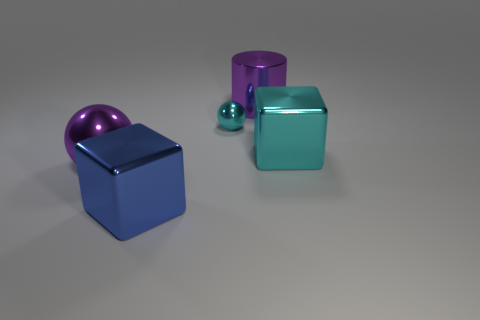
\includegraphics[width=.8\linewidth]{figures/CLEVR_extended_example.png}
  \caption{Example of a generated image with the extended code}
  \label{fig:clevr-extended_example}
\end{figure}

The extended version of the dataset divides the objects into \emph{target object} and \emph{distractors}. The target object is the main object in the scene that should be identified and communicated by the agents. The distractors contain similar objects to the target object. The number of shared attributes is defined by rules researched in \citet{Dale1995}. The target object is therefore always identifiable using either only the \emph{shape} (1), the \emph{shape} and \emph{color} (2) or the \emph{shape}, \emph{color} and \emph{size} (3).

For this research, two datasets are created. The \emph{DaleTwo} dataset contains one target object and one distractor, while the \emph{DaleFive} dataset contains one target object and four distractors. Both datasets contain 10.000 images. For each image fixed size bounding boxes around each object are extracted. These bounding boxes are the input for the sender and receiver in the language game.

\subsection{Language game}
The language game was developed and run in the EGG framework \citep{Kharitonov2019}. The setup of the game is based on the game described in the paper by \citet{Lazaridou2016}. The same multiple images are passed to a sender and a receiver. The sender must communicate the target image to the receiver with a message, who needs to identify this target image. Instead of distinguishing two images from different concepts, in this experiment the agents need to distinguish two objects with shared attributes. Both sender and receiver have a similar architecture to the \emph{agnostic sender} and \emph{receiver} in \citet{Lazaridou2016}. One central difference is the production of the message. Their paper focuses on the classification of a concept for the input image and therefore produces only one-symbol messages that should correspond to these concepts. This research focuses on the identification of attributes for the objects and their combination, which is why our models produce a sequence of symbols for the message (which may correspond to the attributes). This is done using an encoder LSTM (sender) and a decoder LSTM (receiver) (see Figure \ref*{todo}).

The initial state of the encoder LSTM is the image, passed through ResNet101 and a following linear layer that reduces the dimensions. The sequence is then created through Gumbel-Softmax relaxation \citep{Jang2016}.

The receiver on the other side takes the sequence as input for its decoder LSTM. The hidden state is randomly initialized. After each step of the LSTM, the receiver calculates the dot product between the hidden state and its own image encoding (calculated as the sender's image encoding). The receiver then 'points' to one of the images, while applying the softmax function over the results. The loss is calculated using the NLL-loss. Following, the losses for each token in the message sequence are summed up, and all weights of the receiver as well as the sender are updated, based on this summed loss.

There are five variables in the experiments that are adjusted: (1) the image embedding size for the sender $e_s$, (2) the LSTM hidden size for the sender $h_s$, (3) the image/message embedding size for the receiver $e_r$, (4) the LSTM hidden size for the receiver $h_r$ and (5) the size of the vocabulary $|V|$.

The results will be evaluated using the accuracy if the receiver could identify the target object. A random guess corresponds to 50\% in the \emph{DaleTwo} dataset and 20\% in the \emph{DaleFive} dataset.

\section{Results}
TODO:
\begin{itemize}
  \item DaleTwo: \textbf{(done)}
        \begin{itemize}
          \item small hidden/embedding dims, small vocab -> high accuracy
          \item high hidden/embedding dims, small vocab -> low accuracy
        \end{itemize}
  \item DaleFive: \textbf{(done)}
        \begin{itemize}
          \item small hidden/embedding dims, small vocab -> low accuracy
          \item small hidden/embedding dims, bigger vocab -> higher accuracy
        \end{itemize}
  \item ... test different hidden/embedding dims
  \item ... test 3/4 objects
\end{itemize}

\begin{table}
  \centering
  \begin{tabular}{c|ccccc|c}
    \hline
    \textbf{Dataset} & $h_{s}$ & $e_{s}$ & $h_{r}$ & $e_{r}$ & $|V|$ & \textbf{Acc.} \\
    \hline
    DaleTwo          & {10}    & {10}    & {10}    & {10}    & {10}  & {95\%}        \\
    DaleTwo          & {50}    & {50}    & {128}   & {128}   & {10}  & {50\%}        \\
    DaleFive         & {10}    & {10}    & {10}    & {10}    & {10}  & {23\%}        \\
    DaleFive         & {10}    & {10}    & {10}    & {10}    & {20}  & {23\%}        \\
    DaleFive         & {10}    & {10}    & {10}    & {10}    & {100} & {41\%}        \\
    \hline
  \end{tabular}
  \caption{Result of the experiments with different hidden sizes, embedding sizes and vocabulary sizes}
  \label{tab:results}
\end{table}

The results of the experiments are summarized in Table \ref{tab:results}. For the \emph{DaleTwo} dataset it can be clearly seen that very small embedding and hidden sizes are beneficial for identifying the correct object. The receiver identifies indeed almost every sample correctly with all sizes of 10. When the hidden and embedding sizes are increased, the guesses by the receiver are random. Interestingly, a vocab size of 10 is enough to communicate a meaningful message for the \emph{DaleTwo} dataset.

The result change, when using the \emph{DateFive} dataset with four distractors. With low hidden, embedding and vocab size, the agents barely pass the random baseline with 23\%. Only increasing the vocabulary size to 100 raises the accuracy by almost 20\% to 43\%. This accuracy is still far lower than the 95\% with the \emph{DaleTwo} dataset.

\section{Discussion}
TODO:
\begin{itemize}
  \item maybe calculation of loss (multiplicating instead of summing loss per token), unlikely, since sequence length short -> shouldn't result in big differences
  \item reducing dims of image better the increasing dims of message, increasing dims is not learnable for models
  \item Vocab:
        \begin{itemize}
          \item vocabulary could describe attributes of target image (non-discriminative) or describe only differences (discriminative)
          \item in second case, two images is a far easier task than five images. Hence, much lower accuracy
        \end{itemize}
\end{itemize}



\section{Conclusions and further work}

\section*{Acknowledgements}

% Entries for the entire Anthology, followed by custom entries
\bibliography{anthology,custom}


\appendix

\section{Example Appendix}


\end{document}